\section{Model of curved 1D magnetic systems}\label{sec:theory_1D}

The theoretical description of the time evolution of magnetization distribution in curved systems is based on the solution of the phenomenological Landau--Lifshitz--Gilbert (LLG) equation of motion
\begin{equation}\label{eq:llg}
\frac{\mathrm{d}\vec{m}}{\mathrm{d}t}=\underbrace{-\gamma_0\, \vec{m}\times\vec{H}_\textrm{eff}}_{\text{Precession term}} + \underbrace{\alpha_\textsc{g}\, \vec{m}\times\frac{\mathrm{d}\vec{m}}{\mathrm{d}t}}_{\text{Damping term}},
\end{equation}
which defines the damped precession motion of the unit magnetization vector, $\vec{m}=\vec{M}/M_s$, with $M_s$ being a saturation magnetization, around an effective magnetic field $\vec{H}_\textrm{eff}=-\delta E/\delta\vec{M}$ with $E$ being total energy. In Eq.~\eqref{eq:llg}, $\gamma_0$ is the gyromagnetic ratio and $\alpha_\textsc{g}$ is the Gilbert damping parameter.

Without losing generality, let us consider the prototypical case of a curvilinear anisotropic 1D Heisenberg nanomagnet, which is determine in the Cartesian frame of reference by a three-dimensional curve $\vec{\gamma}=\vec{\gamma}(s)$ with $s$ being the natural parameter\footnote{It means that $|\partial_s\vec{\gamma}|=1$.}. The total energy of such magnet includes energies of exchange interaction $E_\textsc{x}$ and uniaxial magnetic anisotropy $E_\textsc{a}$
\begin{equation}\label{eq:total_energy}
E=E_\textsc{x} + E_\textsc{a} =\int\mathrm{d}\vec{r}\, \left[A \, (\nabla m_i)(\nabla m_i)-K \, (\vec{m}\cdot \vec{e}_\textsc{a})^2 \right].
\end{equation}
Here and below we will use the Einstein summation convention with $i = x,\,y,\,z$. The first term in Eq.~\eqref{eq:total_energy} describes the isotropic exchange interaction with $A$ being the exchange stiffness constant, while the second term corresponds to the magnetic anisotropy with $K$ and $\vec{e}_\textsc{a}$ being the constant and the direction of the uniaxial anisotropy, respectively. The competition between exchange and anisotropy results in the magnetic length $\ell=\sqrt{A/K}$, which determines a length scale of the system.

In the case of an arbitrary curved magnetic wire and tangential direction of the anisotropic easy-axis\footnote{It is known~\cite{Hillebrands06} that for thin wires of circular and square cross sections the magnetostatic energy is reduced to an effective easy-tangential shape anisotropy, including the case of a curvilinear wire~\cite{Slastikov12}. In this case the magnetostatic interaction results in the shift of the anisotropy constant $K\to K^\text{eff} = K + \pi M_s^2$.}, i.e. $K>0$ and $\vec{e}_\textsc{a} = \vec{e}_\textsc{t}$, the consideration of magnetic anisotropy becomes non-trivial due to the coordinate-dependence of its term in Eq.~\eqref{eq:total_energy}. Therefore, it is instructive to introduce a local curvilinear frame of reference, which allows to restore the translation-invariant form of $E_\textrm{an}$ and get rid of the coordinate dependence in the anisotropy term. In the case of 1D systems, it is convenient to use the Frenet--Serret reference frame  
\begin{equation} \label{eq:Frenet-Serret}
\vec{e}_\textsc{t} =\partial_s \vec{\gamma}, \qquad  \vec{e}_\textsc{n} =\partial_s \vec{e}_\textsc{t}/|\partial_s \vec{e}_\textsc{t}| , \qquad  \vec{e}_\textsc{b} = \vec{e}_\textsc{t} \times \vec{e}_\textsc{n},
\end{equation}
where $\vec{e}_\textsc{t}$, $\vec{e}_\textsc{n}$, and $\vec{e}_\textsc{b}$ are the tangential, normal, and binormal unit vectors, respectively, see Fig.~\ref{fig:TNB}. The relation between $\partial_s\vec{e}_{\alpha}$ and $\vec{e}_{\alpha}$ is determined by the Frenet--Serret formulas~\cite{Kreyszig91}
\begin{equation} \label{eq:FrenetSerret_basis}
\partial_s\vec{e}_{\alpha} = \mathcal{F}_{\alpha \beta} \, \vec{e}_{\beta}, \qquad \begin{Vmatrix} \mathcal{F}_{\alpha \beta} \end{Vmatrix} = \left(\begin{matrix*} \, 0 \quad	& \kappa \quad &  0 \, \, \, \\ \, -\kappa \quad & 0 \quad & \tau \, \, \, \\
\, 0 \quad & -\tau \quad &	0 \, \, \,
\end{matrix*}\right).	
\end{equation}
Here, Greek indices $\alpha,\, \beta = \textrm{T},\, \textrm{N},\, \textrm{B}$ enumerate the curvilinear coordinates and the curvilinear components of vector fields, $\kappa(s)$ and $\tau(s)$ are local curvature and torsion of the wire, respectively. Using the introduced Frenet--Serret frame of reference it is now possible to parameterize physical wires/stripes with a finite cross section as
\begin{equation} \label{eq:Stripe_param}
\vec{r}\left(s,\zeta_1,\zeta_1\right)=\vec{\gamma}(s) + \zeta_1 \, \vec{e}_\textsc{n}+\zeta_2 \, \vec{e}_\textsc{b},
\end{equation}
where $\zeta_i$ are coordinates within the cross section, see Fig.~\ref{fig:TNB}. In the case when $\sqrt{\zeta_1^2+\zeta_2^2}\leq \ell$, the magnetic object can be treated as a 1D system with~$\vec{m}=\vec{m}(s)$.

%==================================================================\
\begin{figure}[t]
	\centering
	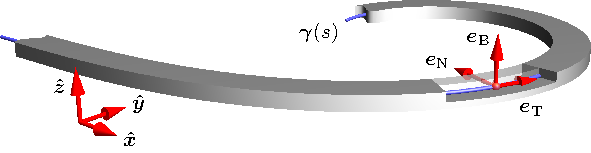
\includegraphics[width=0.7\textwidth]{fig_TNB_basis}
	\caption{\label{fig:TNB}%
		\textbf{Schematics of Frenet--Serret basis for flat curvilinear geometries.} Geometrical construction of a flat curved system from the one-dimensional wire $\vec{\gamma}(s)$ by using geometrical expansion along normal $\vec{e}_\textsc{n}$ and binormal $\vec{e}_\textsc{b}$ directions. 
	}
\end{figure}
%==================================================================/

Applying the Frenet--Serret apparatus~\eqref{eq:Frenet-Serret} to any kind of curved 1D magnetic nanowire leads to the restoring of the translational-invariant form of magnetic anisotropy and restructuring all magnetic energy terms containing spatial derivatives. In this case, the exchange interaction is becoming a characteristic example of such geometrical transformation: in the curvilinear reference frame~\eqref{eq:Frenet-Serret} with the magnetization parametrization $\vec{m} = m_\textsc{t}\,\vec{e}_\textsc{t} + m_\textsc{n}\,\vec{e}_\textsc{n} + m_\textsc{b}\,\vec{e}_\textsc{b}$, the exchange energy reads as~\cite{Sheka15}:
\begin{equation} \label{eq:Exchange_energy_TNB_1}
E_{\textsc{x}} = S \, \int \textrm{d} s  \, \, A \left[\partial_s m_\alpha \partial_sm_\alpha + \mathcal{F}_{\alpha \beta} \, ( m_{\alpha} \, \partial_s m_{\beta} - \partial_s m_{\alpha} \, m_{\beta} ) + \mathcal{K}_{\alpha \beta} \, m_{\alpha} \, m_{\beta} \right],
\end{equation}
where $S$ is the cross section area of the nanomagnet. The first term is the isotropic part of the exchange which formally  has the same form as for a straight wire. The second term in \eqref{eq:Exchange_energy_TNB_1} is the chiral term, which has the set of the Lifshitz invariants and describe the geometrical symmetry breaking. This set of the Lifshitz invariants in the curvilinear frame of reference can be referred to a curvature-induced Dzyaloshinskii--Moriya interaction (DMI), which is linear with respect to local curvature $\kappa(s)$ and torsion $\tau(s)$. The third term in \eqref{eq:Exchange_energy_TNB_1} describes the curvature-induced anisotropy. The corresponding coefficients are determined by the components of the tensor $\mathcal{K}_{\alpha \beta}= \mathcal{F}_{\alpha \nu} \, \mathcal{F}_{\beta \nu}$, which are bilinear with respect to local curvature $\kappa$ and torsion $\tau$
\begin{equation} \label{eq:K_tensor_exchange}
\begin{Vmatrix} \mathcal{K}_{\alpha \beta} \end{Vmatrix} = \left(\begin{matrix*}  \, \kappa^2 \quad	& 0 \quad & - \kappa \, \tau \, \,  \\
\, 0 \quad & \kappa^2 + \tau^2 \quad & 0 \, \,  \\
\, - \kappa \, \tau \quad & 0 \quad &	\tau^2 \, \, 
\end{matrix*}\right).
\end{equation}
It is also convenient to represent the exchange energy \eqref{eq:Exchange_energy_TNB_1} in the following form
\begin{equation} \label{eq:Exchange_energy_TNB_2}
E_{\textsc{x}} =  S \, \int \textrm{d} s \, \, A \left| \partial_s \vec{m} \right|^2 - S \int \textrm{d} s \, \, \vec{D}^{\scriptsize \textsc{e}} \cdot [\vec{m} \times \partial_s\vec{m}] - S \int \textrm{d} s \, \, A \left[ \tau \, m_{\scriptsize \textsc{t}}  + \kappa \, m_{\scriptsize \textsc{b}} \right]^2, 
\end{equation}
where the constraint $|\vec{m}|=1$ and Frenet--Serret formulae are utilized. In the~\eqref{eq:Exchange_energy_TNB_2}, vector $\vec{D}^{\scriptsize \textsc{e}} = - 2 \, A \, \tau \, \vec{e}_{\scriptsize \textsc{t}} - 2 \, A \, \kappa \, \vec{e}_{\scriptsize \textsc{b}}$ denotes to the the \textit{extrinsic} curvature-driven DMI vector~\cite{Gaididei14,Sheka15,Sheka15c}.	In contrast to the \textit{intrinsic} DMI, which comes from the spin-orbit coupling in bulk magnetic crystals with low symmetry~\cite{Dzyaloshinsky58,Moriya60a} or at interfaces between a ferromagnet and a nonmagnetic material with strong spin-orbit coupling~\cite{Fert90,Crepieux98,Bode07,Yang15}, the strength of \textit{extrinsic} DMI is determined by local curvature and torsion~\cite{Pylypovskyi16,Volkov19c}. The vector of the \textit{extrinsic} DMI is always lying in the rectifying TB plane to a curved geometry~\cite{Volkov18}.

For sake of simplicity, in the following we will work in the dimensionless units, for details see Table~\ref{tab:notation}.

%==================================================================\
\begin{table}[h!]
	\begin{tabular}{p{0.25\columnwidth}p{0.35\columnwidth}p{0.35\columnwidth}}
		\hline\hline
		Notation & Dimensionless quantity & Unit of measurement \\
		\hline
		$\vec{m}=\vec{M}/M_s$ & Magnetization & $M_s$\\
		$\xi = s /\ell$ & Length & $\ell = \sqrt{A/K}$\\
		$\overline{t} = t\omega_0$ & Time & $\omega_0 =2 \gamma_0 K / M_s$\\
		$\mathcal{E}=E/E_0$ & Energy & $E_0=S\sqrt{AK}$\\
		$\varkappa = \kappa \ell$ & Curvature & $\ell = \sqrt{A/K}$\\
		$\Omega = \omega/ \omega_0$ & Frequency & $\omega_0 =2 \gamma_0 K / M_s$\\
		$f' = \partial_\xi f$ & Derivative with respect to $\xi$ &\\
		$\dot{f}= \partial_{\overline{t}} f$ & Derivative with respect to $\overline{t}$ & \\
		\hline\hline
	\end{tabular} 
	\caption{\label{tab:notation} Notations and units of measurement used in this chapter.}
\end{table}
%==================================================================/